\section{L-system grammars}

According to Prusinkiewicz and Hanan a simple type of L-systems are those known as deterministic 0L systems, where the string refers to the sequence of cellular states and '0L system' abbreviating 'Lindenmayer system with zero-sided interactions'.  With 0L systems there are only three major parts. There is a set of symbols (\textit{alphabet}), the starting string (\textit{Axiom}) and state transition rules (\textit{rules}). The alphabet is a set of states. The starting string is a starting point containing one or more states. The transition rules are rules that dictate whether a state should remain the same or transition into a different state or even disappear. \cite{prusinkiewicz2013lindenmayer}. \\
\\
An example of a deterministic 0L system is that a simplified model for the growth of algae: \\
\\
We are given the \textit{alphabet}: A, B \\ 
and the \textit{axiom}: A \\
and the \textit{rule} set: \\ 
A $\rightarrow$ AB \\
B $\rightarrow$ A \\
\\
If we then apply the rules to the L-system we find it creates the following generation structure. \\
1.) A \\
2.) AB \\
3.) ABA \\
4.) ABAAB \\
5.) ABAABABA \\
6.) ABAABABAABAAB \\
\\
This rewriting of initial string using a set of rules is ultimately the underlying concept behind L-systems. There are a number of improvements that can be made to this type of L-system in order to accommodate for more complex and intricate structure. One of which is the inclusion of \textit{constants}. Constants can be considered any state that does not have a rule associated with it or remains the same from generation to generation and therefore holds a consistent value or meaning. These constants are used when the L-system is interpreted and thus holds a constant value during string rewriting.


\section{Interpreting L-systems}

Once we have generated the set of rules that allow us to create the L-system we are left with a string of characters which represent that particular L-system. As with any grammar, there is a number of ways of interpreting the string that is generated by the L-systems rules. One method proposed by Przemyslaw Prusinkiewics is "to generate a string of symbols using an L-system, and to interpret this string as a sequence of commands which control a 'turtle'". \cite{prusinkiewicz1986graphical}
\\
\\
A two dimensional L-system string may hold the following commands in the form of symbols. \\
\\
$\bullet$ F: 				\hspace{10mm} 		Move forward by a specified distance whilst drawing a line \\
$\bullet$ f: 				\hspace{10mm} 		Move forward by a specified distance without drawing a line \\
$\bullet$ +: 				\hspace{10mm} 		Rotate to the right specified angle. \\
$\bullet$ -: 				\hspace{10mm} 		Rotate to the left by a specified angle.  \\
$\bullet$ $[$: 				\hspace{10mm} 		Save the current position and angle. \\
$\bullet$ $]$: 				\hspace{10mm} 		Load a saved position and angle. \\
\\
Similarly a three dimensional L-system string may hold the following commands in the form of symbols. \\
\\ 
$\bullet$ F: 				\hspace{10mm}  		Move forward by a specified distance whilst drawing a line \\
$\bullet$ f: 				\hspace{10mm} 		Move forward by a specified distance without drawing a line \\
$\bullet$ +: 				\hspace{10mm} 		Yaw to the right specified angle. \\
$\bullet$ -: 				\hspace{10mm} 		Yaw to the left by a specified angle.  \\
$\bullet$ /: 				\hspace{10mm} 		Pitch up by specified angle. \\
$\bullet$ $\backslash$: 	\hspace{10mm} 		Pitch down by a specified angle.  \\
$\bullet$ $\hat{}$: 		\hspace{10mm} 		Roll to the right specified angle. \\
$\bullet$ \&:				\hspace{10mm}  		Roll to the left by a specified angle.  \\
$\bullet$ $[$: 				\hspace{10mm} 		Save the current position and angle. \\
$\bullet$ $]$: 				\hspace{10mm}		Load a saved position and angle. \\

\begin{figure}[htbp]
	{\centering
		\vspace{7px}
		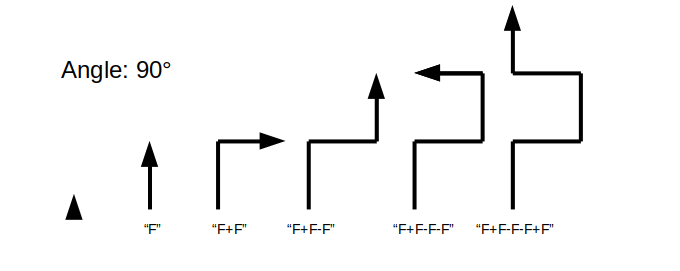
\includegraphics[scale=0.5]{Diagrams/basic_turtle.png}
		\caption{Diagram showing a turtle interpreting simple L-system string.}
	}
\end{figure}
\FloatBarrier

\section{Branching Filaments}

Explain how branching works and how it can be used for generating the L-systems

\begin{figure}[htbp]
	{\centering
		\vspace{7px}
		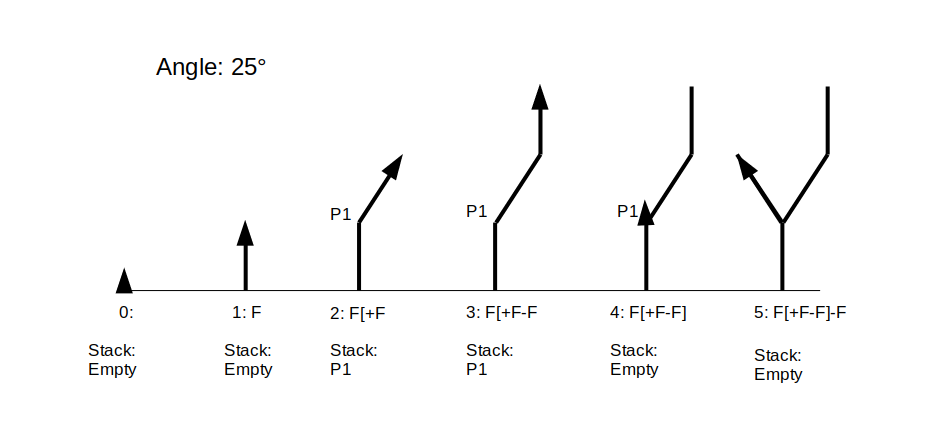
\includegraphics[scale=0.5]{Diagrams/branching_turtle.png}
		\caption{Diagram showing a turtle interpreting an L-system incorporating branching.}
	}
\end{figure}
\FloatBarrier


\section{Basic 2D L-systems} 

There are a number of fractal geometry that have become well known particularly with regards to how they can seemingly imitate nature \cite{mandelbrot1982fractal}. Particularly with the geometry such as the Koch snowflake which can be represented using the following L-system.

\begin{figure}[htbp]
	\raggedright
	\textbf{\underline{Koch Curve:}} \\
	\textbf{Alphabet:} F \\
	\textbf{Constants:} +, - \\
	\textbf{Axiom:} F \\
	\textbf{Angle:} 90$^\circ$ \\
	\textbf{Rules:} \\
	F $\rightarrow$ F+F--F+F\\
	{\centering
		\vspace{7px}
		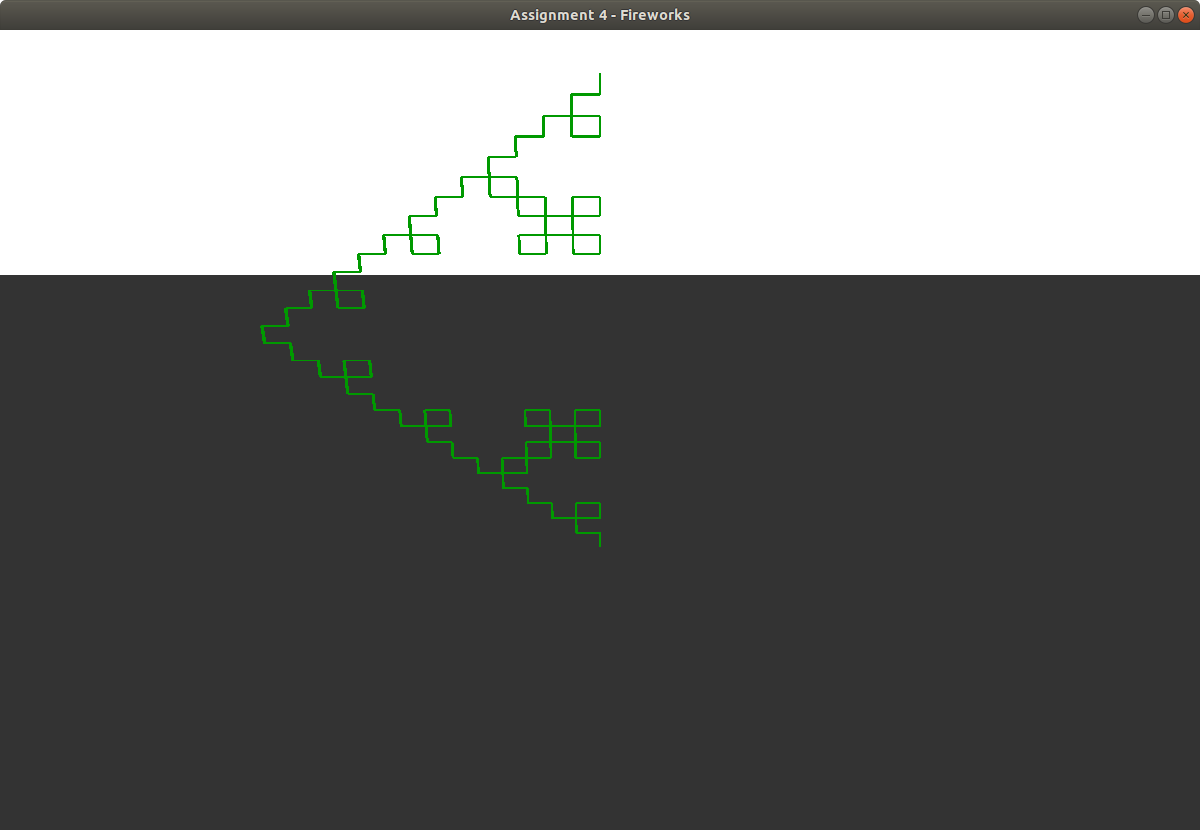
\includegraphics[scale=0.8]{KochCurve/KochCurve04.png}
		\caption{Koch Curve.}
	}
\end{figure}
\begin{figure}[htbp]
	\raggedright
	\textbf{\underline{Sierpinski Triangle:}} \\
	\textbf{Alphabet:} A, B \\
	\textbf{Constants:} +, - \\
	\textbf{Axiom:} A \\
	\textbf{Angle:} 60$^\circ$ \\
	\textbf{Rules:} \\
	A $\rightarrow$  B-A-B \\
	B $\rightarrow$ A+B+A\\
	{\centering
		\vspace{7px}
		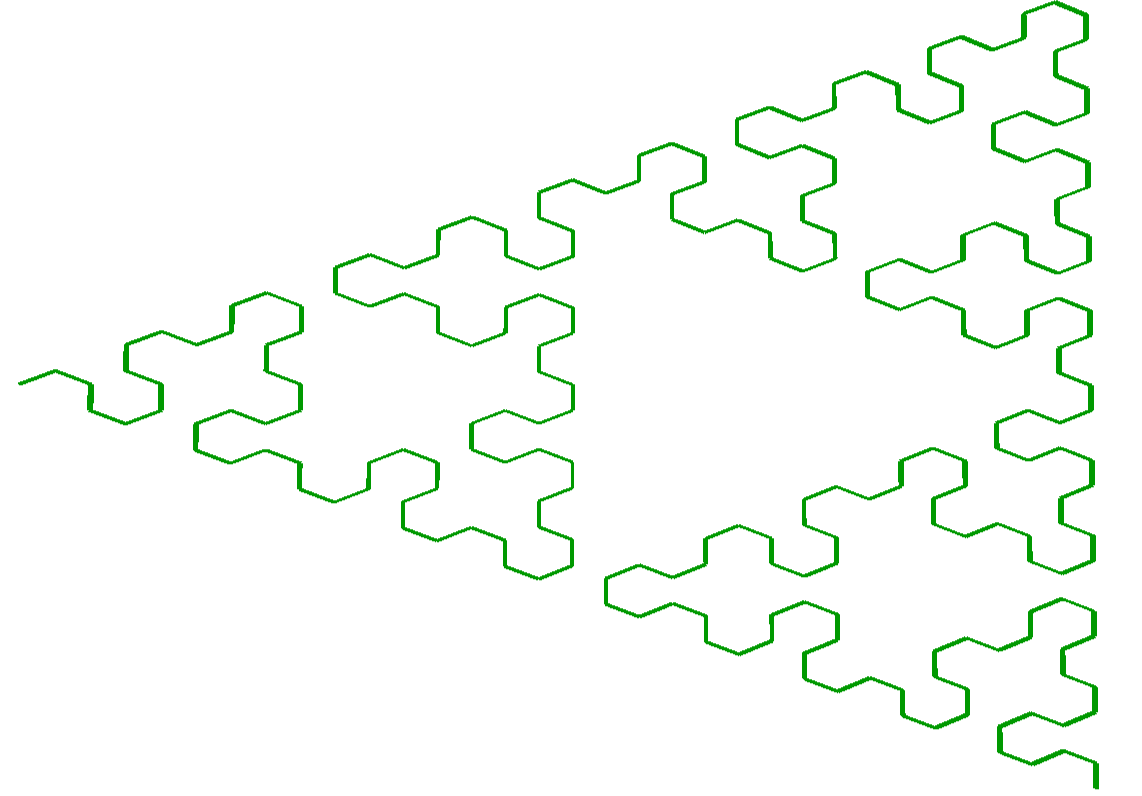
\includegraphics[scale=0.17]{SierpinskiTriangle/SierpinskiTriangle06.png}
		\caption{Sierpinski Triangle.}
	}
\end{figure}
\begin{figure}[htbp]
	\raggedright
	\textbf{\underline{Dragon Curve:}} \\
	\textbf{Alphabet:} F, X, Y \\
	\textbf{Constants:} +, - \\
	\textbf{Axiom:} FX \\
	\textbf{Angle:} 90$^\circ$ \\
	\textbf{Rules:} \\
	X $\rightarrow$ X+YF+ \\
	Y $\rightarrow$ -FX-Y\\
	{\centering
		\vspace{7px}
		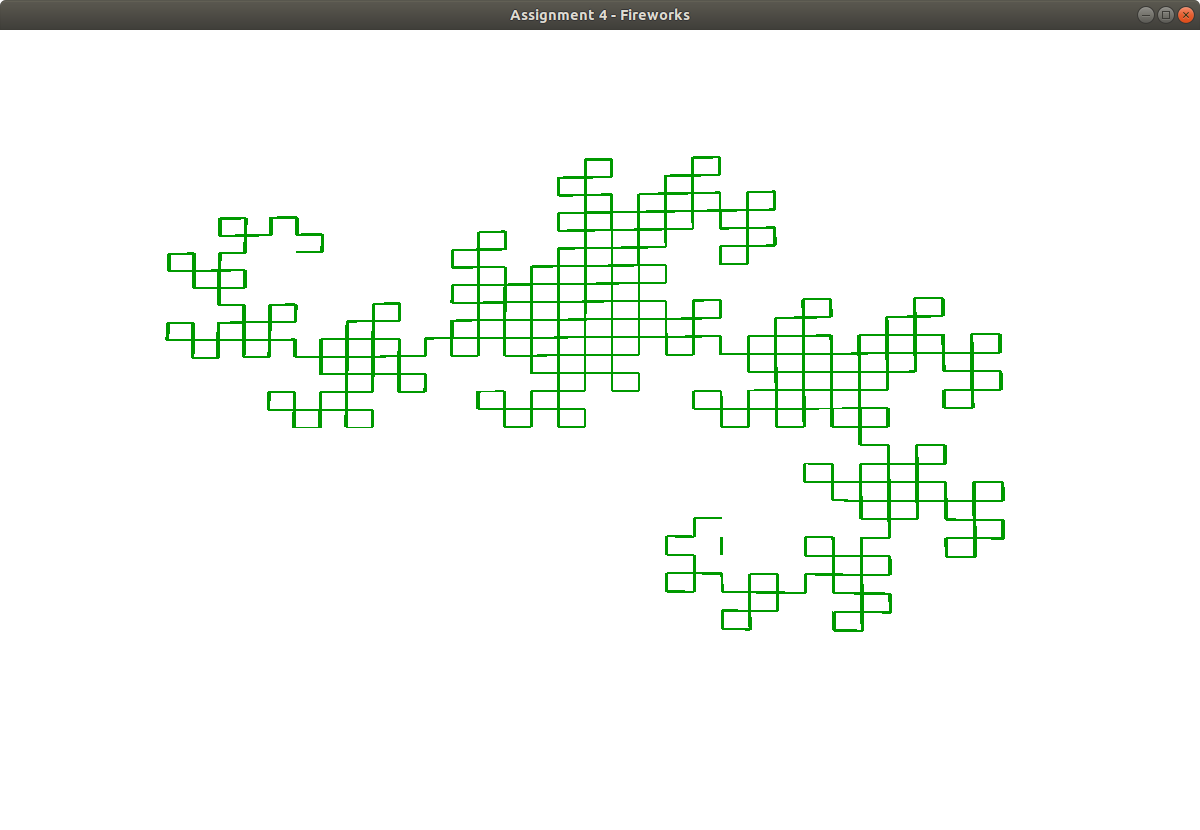
\includegraphics[scale=0.17]{DragonCurve/DragonCurve10.png}
		\caption{Dragon Curve.}
	}
\end{figure}
\begin{figure}[htbp]
	\raggedright
	\textbf{\underline{Fractal Plant:}} \\
	\textbf{Alphabet:} X, F\\
	\textbf{Constants:} +, -, [, ] \\
	\textbf{Axiom:} X \\
	\textbf{Angle:} 25$^\circ$ \\
	\textbf{Rules:} \\
	X $\rightarrow$ F-[[X]+X]+F[+FX]-X\\
	F $\rightarrow$ FF \\
	{\centering
		\vspace{7px}
		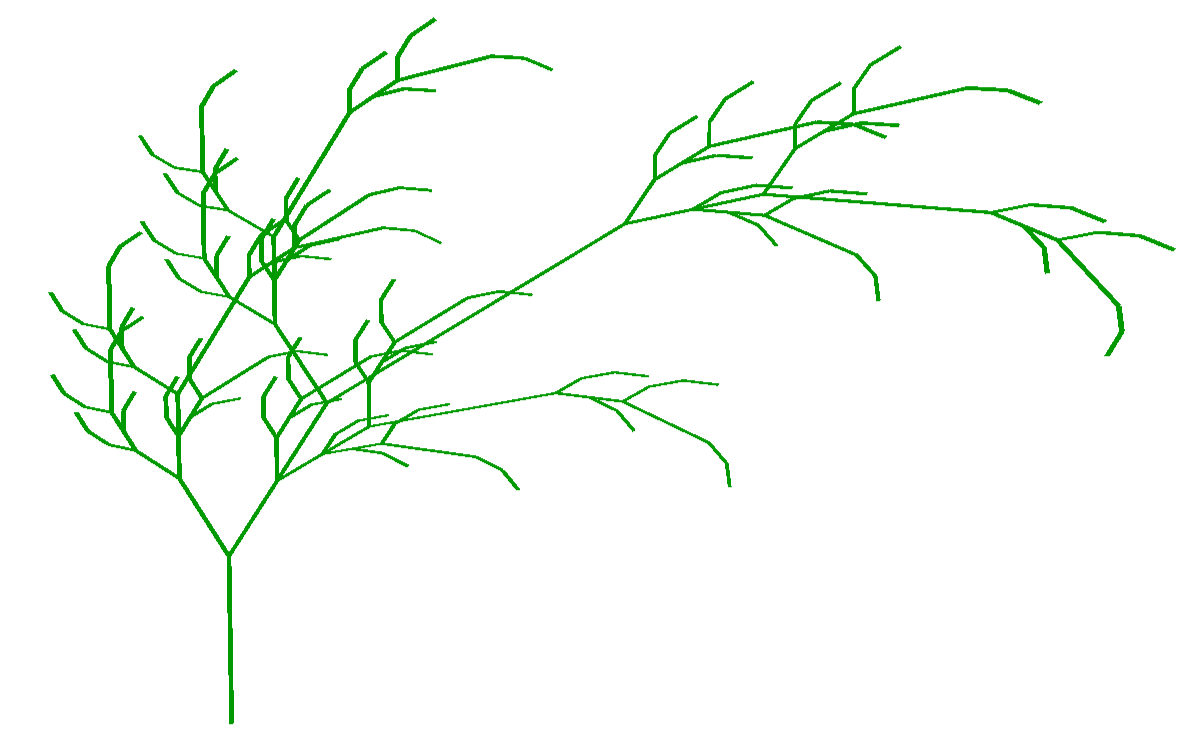
\includegraphics[scale=0.15]{FractalPlant/FractalPlant05.png}
		\caption{Fractal Plant.}
	}
\end{figure}
\begin{figure}[htbp]
	\raggedright
	\textbf{\underline{Fractal Bush:}} \\
	\textbf{Alphabet:} F\\
	\textbf{Constants:} +, -, [, ] \\
	\textbf{Axiom:} F \\
	\textbf{Angle:} 25$^\circ$ \\
	\textbf{Rules:} \\
	F $\rightarrow$ FF+[+F-F-F]-[-F+F+F]\\
	{\centering
		\vspace{7px}
		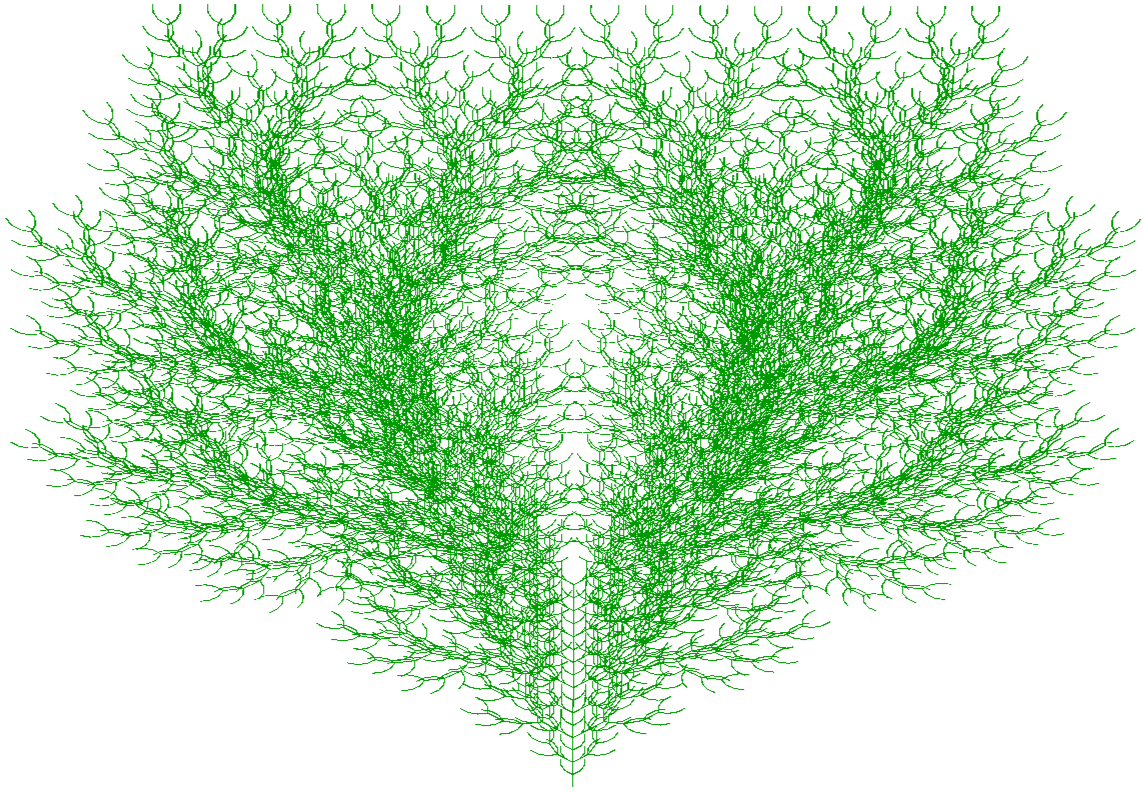
\includegraphics[scale=0.15]{FractalBush/FractalBush06.png}
		\caption{Fractal Bush.}
	}
\end{figure}

\FloatBarrier
\newpage

\section{The Use of L-systems in 3D applications}

L-systems have been talked about and researched since its inception in 1968 by Aristid Lindenmayer. Over the years it's usefulness in modelling different types of plant life has been very clear, however its presence has been quite absent from any mainstream game engines for the most part, these engines relying either on digital artists skill to develop individual plants or on 3rd party software such as SpeedTree. These types of software use a multitude of different techniques however their methods are heavily rooted in Lindenmayer Systems. 

